\chapter{Interactive Teaching}
As we have seen in our sample lesson plans, there are times when a teacher will be lecturing.  However, lecturing to students for whom English is a second or even third language needs to be engaging and visual.  We can not use the same lecture style we were raised on. We knew English and also how to take notes while listening. Instead, we should use interactive teaching techniques to keep our students interested, help them  understand, and improve their English. \\

Interactive lecturing means that although the teacher may at points be the lead speaker, students are still answering questions, asking questions, and focused on the topic at hand.\\

The following suggestions may be helpful in practicing Interactive Teaching:

\section{Learn definitions in a fun way}
Instead of just reading a definition aloud and hoping students will memorize it, help them commit it to memory.  Try reading the definition one student, one word at a time.  This involves all students in the class, makes them speak up, and keeps them paying attention.  Additionally, you can have students break into groups and race to unscramble a definition that has been written word by word on manila paper.\\

\section{Ask Questions}
By asking our students questions, we can access their understanding, build their confidence, and get them speaking English. Try these techniques to get your students answering questions:
\begin{itemize}
\item Start the class each day with review questions from the lesson before to get students' mind on the topic at hand and build their confidence before they enter a new subject.
\item Once the notes are written on the board, ask students questions from the notes, like ``Who can tell me, what are the three types of locomotion?'' rather than students or instructor just reading the notes allowed.
\item Ask questions that call for a choral responses.
\item When a student answers a question, ask the rest of the class if they are correct or incorrect.
\item Have one student answer a question, then have them ask another student a different question.
\item Have students come to the front and face the class to answer questions.
\item Trying using a question ball.
\item Write a question on the board and have students come to the board to answer, then they write a question and have another student answer it.
\end{itemize}

\section{Give Participation Points}
To encourage students answering questions and reading aloud, give a point in the top hand corner of the board every time someone volunteers.   This works very well for girls empowerment and is discussed more in Chapter 8.\\

\section{Be Visual}
When teaching in a foreign language, we should try to be as visual as possible.  Use pictures and examples whenever possible.  If you are teaching about classification, draw the organisms and quiz students.  Common accidents in the chemistry lab could also be drawn and used to teach students the hazards and new English vocabulary.   Teach students shapes by drawing them rather than their Kiswahili name.\\ 

\section{Be Active}
Some topics may be difficult for students to grasp, especially while learning in a new language.  Act out things and get the kids involved whenever possible.  If you are talking about hearing, ask students to touch their ears.  When describing a lever, move your arm.  If you are discussing temperature regulation, have students act like they are in a hot/cold environment.\\  

\begin{figure}[h!]
\centering
\setlength\fboxsep{0pt}
\setlength\fboxrule{2pt}
\fbox{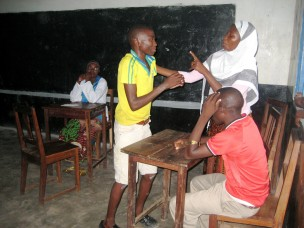
\includegraphics[scale=0.3]{./img/IMG_5127.JPG}} 
\caption{Students acting out the negative effects of Drug Abuse}
\end{figure}

\section{Repeat Difficult Words}
When you are lecturing, note words that might be difficult to say and have the students repeat the word out loud.  Its wakes them up, they practice pronunciation, and they love doing it.\\
Additionally, you can have students spell out the pronunciation of difficult words.

\section{Group Work}
Group work facilitates learning.  Teachers need to organize small groups of students and then teach the students how to work together and help each other learn. All students should be writing and active in the learning, not just one student.  The teacher should guide students to stay on task and move around the room to observe students' progress and give praise. If a group is working too slowly, another student can come to that group to help teach.  When groups are finished, questions answered are (or work done
is) shared and discussed as a class.\\

Questions can also be written on card paper and handed to small groups to be discussed. They can then be passed on to another group.  These cards can also be used like a scavenger hunt.  Groups get one question and when they answer it correctly, they get another question to answer.  The first group to answer all their questions wins.

\section{Critical Thinking}
Critical thinking is key to each lesson.  New material is not given to memorize but to understand and be used. Critical thinking is the process of analyzing, comparing, processing, and using new information. When teaching, ask your students critical thinking questions from the material you presented.  Have students present debates on topics when possible.  Ask students to make a list of scientific questions they have about a topic and then discuss them as a group.

\section{Projects}
Giving students projects allows the students to teach themselves and determine what information is important. Using your school's library, teach students how to use the table of contents and index to find information. Once they create their project, have them present and teach other students. You can also bind the project papers together into a book (1000/=) and put in the library for future use and to create pride in students' work.
